% Preamble
\documentclass[11pt]{scrartcl}

    % Packages
    \usepackage{a4wide}
    \usepackage[utf8]{inputenc}
    \usepackage[T1]{fontenc}
    \usepackage[naustrian]{babel}
    \usepackage{lmodern}
    \usepackage{microtype}
    
    \usepackage{verbatim}
    \usepackage{enumerate}
    \usepackage{scrextend}
    \usepackage{graphicx}
    \usepackage{parskip}
   	\usepackage[dvipsnames]{xcolor}
    \usepackage{tikz}
   
    \usepackage{amsmath}
    \usepackage{amsfonts}
    \usepackage{amssymb}
        
    \title{Rechnerorganisation - 2.\ Klausurvorbereitung}
    \author{Auer Thomas, Stefan Haan}
    \date{\today}

\begin{document}
\maketitle
\tableofcontents
\graphicspath{{graphics/}}

\setcounter{section}{4}
\pagebreak

\section{Übungsblatt 5}
    \subsection{Multi-Cycle Datenpfad: lw-Instruktion}
    \textbf{Erläutern Sie die Ausführung der lw-Instruktion (load word) für den Multi-Cycle-Datenpfad.
    Welche Vorteile bietet der Multi-Cycle-Datenpfad gegenüber dem Single-Cycle-Datenpfad?
    Diskutieren Sie dies anhand dieses Befehls.}

  %  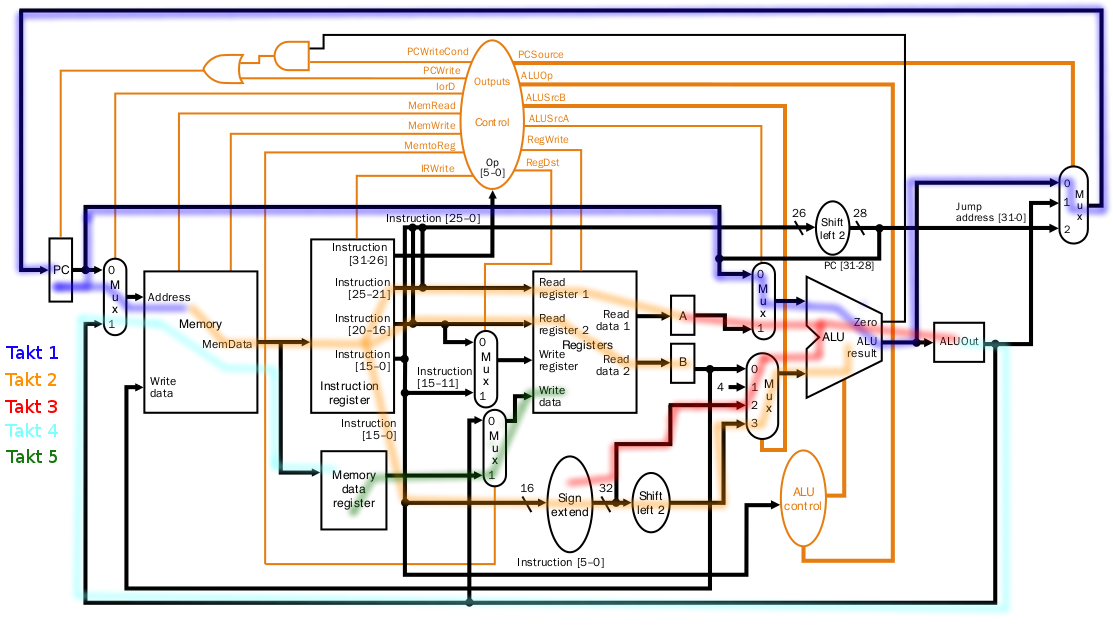
\includegraphics[width=\textwidth]{LW_MCDp}

    \subsection{Grundlagen Pipelining}
    \textbf{Gegeben seien vier unterschiedliche Prozessoren, die sich in der Anzahl der Pipelinestufen und
    der Taktrate unterscheiden:\\}
    \begin{center}
        \begin{tabular}{l|l|l}
        Prozessor & Pipelinestufen & Taktrate \\\hline
        A & 1 & 100 MHz \\
        B & 4 & 800 MHz \\
        C & 12 & 1,5 GHz \\
        D & 20 & 3,2 GHz \\
        \end{tabular}
    \end{center}
    \textbf{(a) Bestimmen Sie für jeden Prozessor die Latenz der einzelnen Instruktionen.}
    
    \textbf{Wie lange dauert die Ausführung von 400.000 voneinander unabhängigen Instruktionen
    auf jedem der angeführten Prozessoren? Bestimmen Sie die Performance und den
    Speedup verglichen mit Prozessor A ohne Pipelining. (Sie können annehmen, dass es
    keine Stalls gibt.)}

    \subsection{Pipelining: Graphische Darstellung}

    \textbf{Beantworten Sie folgende Fragen anhand der Beispiel-Pipeline-Architektur der VO (Kapitel 3.2).\\\\
    (a) Bestimmen Sie die Anzahl der Pipelinestufen, die Taktdauer und die Taktfrequenz der
    Beispiel-Pipeline unter Annahme der Angaben auf VO-Folie 3-44 (Ausführungszeiten der
    Funktionseinheiten). Wie lange dauert die Ausführung eines einzigen Befehls auf der
    Beispiel-Pipeline?\\\\
    (b) Angenommen es treten keine Leertakte (stalls) auf, welchen Speedup erreicht die
    Beispiel-Pipeline aus a) gegenüber einem Single-Cycle Datenpfad, der aus den gleichen
    Funktionsregistern besteht?\\
    Seite 1 von 2\\\\
    (c) Auf der Pipeline wird folgende Befehlssequenz ausgeführt:\\}
    \begin{verbatim}
        and     $10, $2, $3
        sw      $11, 4($3)
    \end{verbatim}

    \textbf{    Stellen Sie die Ausführung der oben angeführten Befehlssequenz durch die Beispiel-Pipeline
    wie auf VO-Folie 3-45 grafisch dar (untere Abbildung). Achten Sie insbesondere auf die
    zeitliche Anordnung der Zugriffe auf die Registereinheit! Wie lange dauert die Ausführung der
    Befehlssequenz?}


    \subsection{Pipelining: Daten- und Kontrollabhängigkeiten}
    \textbf{Gegeben sei folgendes Code-Fragment:}

    \begin{center}
        
%    \includegraphics[width=0.5\textwidth]{5_4}
    
    \end{center}


\pagebreak
\section{Übungsblatt 6}
\setcounter{subsection}{4}
\subsection{Loop Unrolling}
Folgendes Codefragment wird auf einen Prozessor mit "`Delayed Branching"' (1 Takt Branch Delay) ausgeführt. Die Latenzen zwischen abhängigen Befehlen sind in Tabelle \ref{tbl:stalls1} aufgelistet.

{
	\ttfamily
	\begin{tabular}{l llll}
		loop: & l.d      & \$f4  & 0(\$t0) &      \\
		      & sub.d    & \$f6  & \$f4    & \$f0 \\
		      & l.d      & \$f8  & 0(\$t1) &      \\
		      & mul.d    & \$f10 & \$f6    & \$f8 \\
		      & add.d    & \$f12 & \$f10   & \$f2 \\
		      & s.d      & \$f12 & 0(\$t2) &      \\
		      & addi     & \$t2  & \$t2    & -8   \\
		      & addi     & \$t1  & \$t1    & -8   \\
		      & addi     & \$t0  & \$t0    & -8   \\
		      & bne \$t0 & \$t4  & loop    &      \\
		      & nop      &       &         &
	\end{tabular}
}

\begin{table}[h!]
	\centering
	\begin{tabular}{lll}
		\hline
		Erzeugender Befehl & Benutzender Befehl & Zwischentakte \\ \hline
		FP ALU operation   & FP ALU operation   & 3             \\
		FP ALU operation   & Store FP double    & 2             \\
		Load FP double     & FP ALU operation   & 1             \\
		Load FP double     & Store FP double    & 0             \\
		Load integer       & Integer operation  & 1             \\
		Load integer       & Branch             & 2             \\
		Integer operation  & Integer operation  & 0             \\
		Integer operation  & Branch             & 1             \\ \hline
	\end{tabular}
	\caption{Latenzen zwischen abhängigen Befehlen}
	\label{tbl:stalls1}
\end{table}

\begin{enumerate}[(a)]
	\item \textbf{Identifizieren Sie alle Daten- und Kontrollabhängigkeiten, die Stalls	verursachen\footnote{ohne Forwarding-Einheit}. Wie viele Taktzyklen werden für die
	Ausführung des gesamten Codes bzw. pro Ergebniselement\footnote{d.h. nur die Schleife}
	benötigt?}

	{
		\ttfamily
		\begin{tabular}{l llll}
			loop:                       & l.d   & \color{blue}\$f4        & 0(\$t0)               &                  \\
			\color{blue} +1 Stall       & sub.d & \color{brown}\$f6       & \color{blue}\$f4      & \$f0             \\
			                            & l.d   & \color{cyan}\$f8        & 0(\$t1)               &                  \\
			\color{brown}+2 Stalls      & mul.d & \color{Mulberry}\$f10   & \color{brown}\$f6     & \color{cyan}\$f8 \\
			\color{Mulberry}+3 Stalls   & add.d & \color{Orange}\$f12     & \color{Mulberry}\$f10 & \$f2             \\
			\color{Orange}+2 Stalls     & s.d   & \color{Orange}\$f12     & 0(\$t2)               &                  \\
			                            & addi  & \$t2                    & \$t2                  & -8               \\
			                            & addi  & \$t1                    & \$t1                  & -8               \\
			                            & addi  & \color{Bittersweet}\$t0 & \$t0                  & -8               \\
			\color{Bittersweet}+1 Stall & bne   & \color{Bittersweet}\$t0 & \$t4                  & loop             \\
			                            & nop   &                         &                       &
		\end{tabular}
	}
	\begin{tabular}{llll}
		\hline
		                & Stalls & Instruktionen & $ \Sigma $ \\ \hline
		Ergebniselement & 9      & 11            & 20         \\ \hline
	\end{tabular}
\end{enumerate}

\section{Übungsblatt 7}


\section{Übungsblatt 8}
\setcounter{subsection}{3}
\subsection{Speicherhierarchien 1}
Tabelle \ref{tbl:hirachy1} gibt die \textbf{Verzögerung} im Falle eines \textbf{erfolgreichen} Zugriffs auf die jeweilige Speicherebene an.

Der durchschnittliche CPI-Wert \underline{ohne} Berücksichtigung der Speicherzugriffe betrage 1,3 (idealer CPI). \textbf{20\%} aller Instruktionen greifen auf den Speicher zu.

\begin{table}[h!]
	\centering
	\begin{tabular}{lll}
		\hline
		Speicherebene & Hitrate & Verzögerung/Takte \\\hline
		L1 & 85\% & 4 \\
		L2 & 75\% & 12 \\
		RAM & 100\% & 236 \\\hline
	\end{tabular}
	\caption{Speicherebenen und Verzögerung in Takten}
	\label{tbl:hirachy1}
\end{table}

\begin{enumerate}[a)]
	\item \textbf{Durchschnittlicher CPI-Wert unter Berücksichtigung der Speicherzugriffe}
	\begin{figure}[h!]
		\centering
		\begin{tikzpicture}
		\node{Instruktionen}[->]{
			child{node{Speicherzugriffe} 
				child{node{L1 Miss}
					child{node{L2 Miss}
						child{node[align=center]{RAM\\\textbf{236 CPI}}}
						edge from parent node[left=3mm]{0.25}
					}
					child[missing]
					child{node[align=center]{L2 Hit\\\textbf{12 CPI}}
						edge from parent node[right=3mm]{0.75}
					}
					edge from parent node[left=3mm]{0.15}
				}
				child[missing]
				child{node[align=center]{L1 Hit\\\textbf{4 CPI}}
					edge from parent node[right=3mm]{0.85}
				}
				edge from parent node[left=3mm]{0.20}
			}
			child[missing]
			child{node[align=center]{Andere\\\textbf{0 CPI}}
				edge from parent node[right=3mm]{0.80}
			}
		};
		\end{tikzpicture}
		\caption{Wahrscheinlichkeiten der Speicherzugriffe mit ihren \textbf{Verzögerungen}}
		\label{fig:prob1}
	\end{figure}

	Berechne die durchschnittliche Verzögerung aus Abbildung \ref{fig:prob1} durch gewichtete Aufsummierung der Knoten.
	\begin{equation}
		\overline{\text{Verzögerung}} = 0.8 \cdot 0 + 0.2 \cdot (0.85 \cdot 4 + 0.15 \cdot(0.75 \cdot 12 + 0.25 \cdot 236)) = 2.72
		\label{eq:avgdelay1}
	\end{equation}
	
	
	Addiere die durchschnittliche Verzögerung zum idealen CPI-Wert um den durchschnittlichen CPI-Wert unter Berücksichtigung der Speicherzugriffe zu erhalten.
	\begin{equation}
		\overline{\text{CPI}_\text{gesamt}} = \overline{\text{Verzögerung}} + 1.3 = 4.02
	\end{equation}
	
	
	\item \textbf{Prozent der Ausführungszeit, die der Prozessor auf Speicherzugriffe warten muss}
	
	Die durch Speicherzugriffe verursachte Verzögerung ist $ \overline{\text{Verzögerung}} = 2.72 $. Berechne das Verhältnis zum durchschnittlichen CPI-Wert.
	\begin{equation}
		\frac{\overline{\text{Verzögerung}}}{\overline{\text{CPI}_\text{gesamt}}} = \frac{2.72}{4.02} \approx 0.677
	\end{equation}
	
	
	\item \textbf{Hitrate des L1-Caches, um einen durchschnittlichen CPI-Wert von 3 zu erhalten}
	
	Die maximale Verzögerung, die nun durch Speicherzugriffe auftreten darf, ist $ \overline{\text{Verzögerung}} = 3 - 1.3 = 1.7 $.
	Man schreibe die Gleichung \ref{eq:avgdelay1} um und löse nach der Hitrate des L1 Caches $ p_\text{L1} $.
	\begin{align}
	\overline{\text{Verzögerung}} = 0.8 \cdot 0 + 0.2 \cdot (p_\text{L1} \cdot 4 + (1- p_\text{L1}) \cdot(0.75 \cdot 12 + 0.25 \cdot 236)) &= 1.7 \\
	 p_\text{L1} \cdot 4 + (1- p_\text{L1}) \cdot 68 &= \frac{1.7}{0.2} \\
	  4 \cdot p_\text{L1} - 68 \cdot p_\text{L1} &= 8.5 - 68 \\
	  p_\text{L1} &= \frac{-59.5}{-64} \\
	  &\approx 0.93
	\end{align}
\end{enumerate}


\section{Übungsblatt 9}


\section{Übungsblatt 10}

    
\end{document}